\section{Resultados y discusión}

Se realizaron mediciones del módulo y la fase de la señal inducida en función de la frecuencia angular  $\omega$ para una muestra Al de espesor fijo y, posteriormente, en función del espesor de la placa para una frecuencia fija de 50 Hz. En ambos casos se compararon los resultados experimentales con las predicciones teóricas del efecto skin, obteniendo la conductividad eléctrica a partir de los ajustes realizados y la profundidad de penetración.

\subsection{Espesor fijo}

Para una placa de aluminio de espesor constante, se estudió la dependencia del módulo de la señal y de la fase en función de $\sqrt\omega$.  Según el modelo teórico del efecto skin, la amplitud del campo debe presentar un decaimiento exponencial de la forma \eqref{eq: modulo-z fijo} mientras que la fase debe presentar una dependencia aproximadamente lineal con $\sqrt\omega$  según \eqref{eq: fase-z fijo}. En la \autoref{fig:espfijo} se muestra el diagrama de Bode correspondiente tanto al módulo como a la fase de la señal. 

\begin{figure} [H]
    \centering
    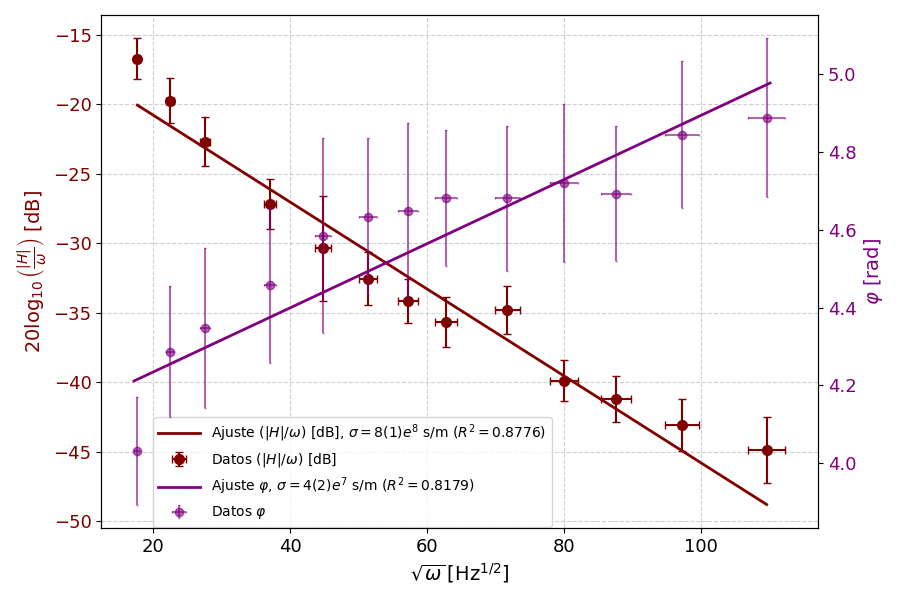
\includegraphics[width=0.7\linewidth]{Figuras 3/espfijo.png}
\caption{Diagrama de Bode de la señal en función de $\sqrt{\omega}$ para espesor fijo. En color borgoña se muestran los datos experimentales correspondientes al módulo junto con su curva de ajuste, y el valor de $\sigma_{|H|}$ obtenido. En color violeta se presentan los datos experimentales de la fase, y su respectivo ajuste junto al valor de $\sigma_{\varphi}$ obtenido.}
    \label{fig:espfijo}
\end{figure}

A partir del ajuste de la fase se obtuvo $\sigma_{\varphi}=4(2)\times10^7$ S/m, valor compatible con lo esperado para la conductividad del aluminio, siendo esta $\sigma_{Al}= 3\times10^7$ S/m. Del ajuste del módulo se obtuvo $\sigma_{|H|}=8(1)\times10^8$ S/m, valor significativamente mayor al esperado y discrepante en más de un orden de magnitud respecto al valor tabulado. No obstante, el comportamiento lineal observado en el gráfico de Bode evidencia una dependencia compatible con la predicción teórica del efecto skin. 

La destacable discrepancia apreciada en para el módulo motivó a comparar el ajuste experimental con una curva teórica según \eqref{eq: modulo-z fijo}, calculada según las características del circuito, que se presenta en \autoref{fig:comparacion} 

\begin{figure} [H]
    \centering
    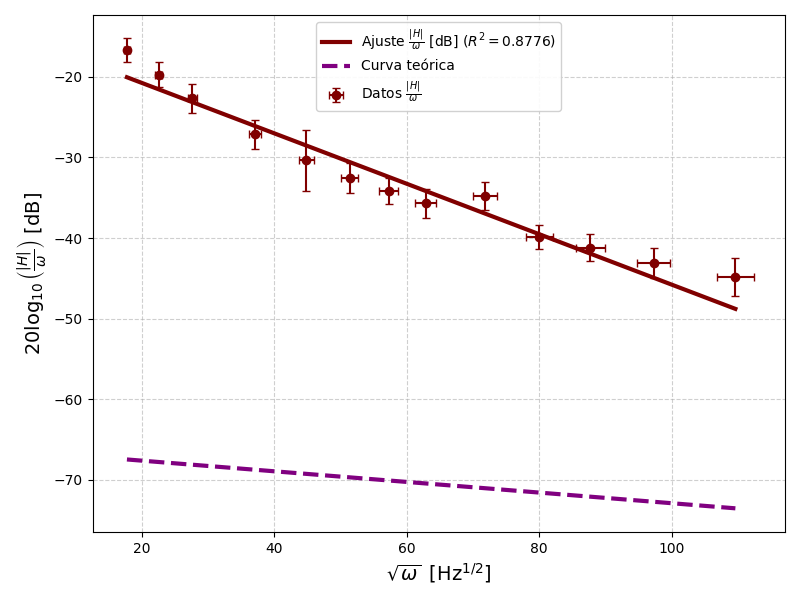
\includegraphics[width=0.7\linewidth]{Figuras 3/comparacion.png}
    \caption{Comparación entre los datos experimentales y su curva de ajuste (en color borgoña) y la respuesta teórica esperada para el sistema (en color violeta).}
    \label{fig:comparacion}
\end{figure}

Se observa que la curva teórica presenta una atenuación considerablemente mayor que la observada experimentalmente. Como consecuencia, el ajuste experimental requiere una profundidad de penetración efectiva menor y conduce a una sobreestimación de la conductividad eléctrica.

Las diferencias observadas pueden atribuirse a diversas limitaciones del modelo teórico utilizado. La expresión empleada supone una geometría unidimensional ideal y un conductor semiinfinito, hipótesis que no se cumplen estrictamente sobre el sistema. La geometría finita de la placa y de las bobinas produce distribuciones no uniformes del campo magnético. Por otro lado, la geometría propia del arreglo experimental genera que parte del flujo magnético generado por el circuito primario no permanezca completamente confinado en el núcleo, existiendo flujo disperso y líneas de campo que atraviesan regiones de aire antes de alcanzar la bobina secundaria, modificando la amplitud de la señal inducida en el bobinado secundario y produciendo contribuciones no contempladas en el modelo teórico. En consecuencia, la determinación de la conductividad a partir del módulo resulta particularmente sensible a efectos geométricos e instrumentales, lo que podría explicar la discrepancia observada en comparación a su homologo obtenido con la fase.
 

\subsection{Espesor variable}

Se realizaron mediciones variando el espesor atravesado por el campo magnético para una frecuencia fija de 50 Hz. Se realizó un bode de la señal en función del espesor $z$ según la representación logaritmica de \eqref{eq: modulo-f fijo} y \eqref{eq: fase-f fijo}, que se muestra en la \autoref{fig:espvar}.

\begin{figure} [H]
    \centering
    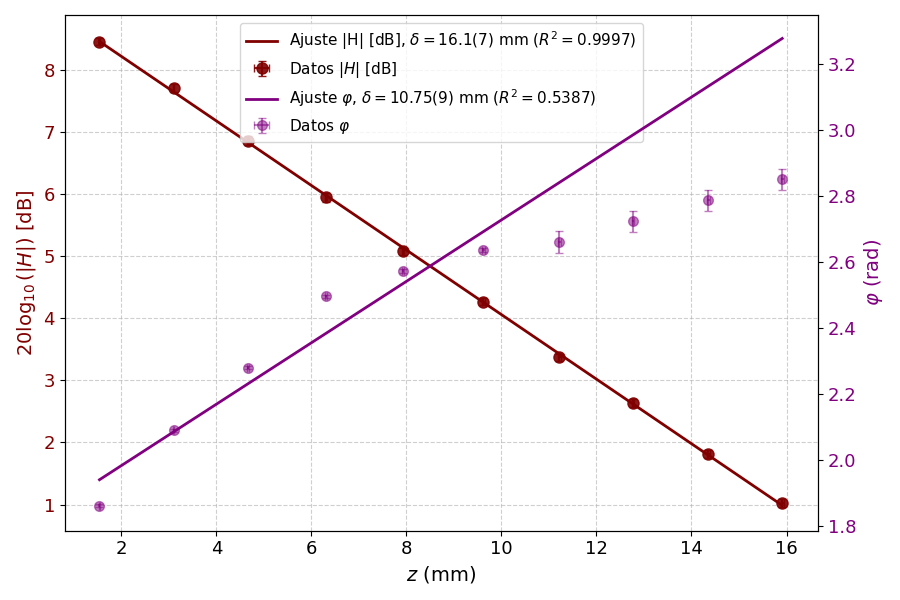
\includegraphics[width=0.7\linewidth]{Figuras 3/espvar.png}
    \caption{Diagrama de Bode de la señal en función del espesor $z$ para frecuencia fija. En color borgoña se muestran los datos experimentales correspondientes al módulo junto con su curva de ajuste, y el valor de $\sigma_{|H|}$ obtenido. En color violeta se presentan los datos experimentales de la fase, y su respectivo ajuste junto al valor de $\sigma_{\varphi}$ obtenido.}
    \label{fig:espvar}
\end{figure}

A partir de la pendiente del ajuste del módulo y utilizando la relación $\delta = \sqrt{\frac{2}{\mu \sigma \omega}}$, se obtuvo una profundidad de penetración $\delta_{|H|}=16.7(1)$ mm. Esta penetración obtenida corresponde a una conductividad $\sigma_{|H|}=1.81(3)\times10^7$ S/m que difiere aproximadamente en un $40\%$ con la referencia. Por otra parte, el ajuste permitió determinar un $\delta_{\varphi}=10.75(9)$ mm. La conductividad asociada fue $\sigma_{\varphi}=4.38(3)\times10^7$ S/m.

Finalmente el promedio ponderado de ambos resultados para la profundidad de penetración es $\delta=13.41(7)$ mm, que, comparado con el valor de referencia para aluminio a $50$ Hz, $\delta_{Al}= 11$ mm, presenta una diferencia porcentual absoluta aproximadamente del $20\%$.
El promedio ponderado para la conductividad es $\sigma=4.26(3)\times10^7$ S/m, presentando una diferencia porcentual absoluta del $13\%$ con la referencia.

De cualquier manera, en ambos casos se observa una concordancia cualitativa con las predicciones del efecto skin: el módulo presenta una disminución aproximadamente lineal en escala logarítmica al aumentar el espesor, mientras que la fase aumenta linealmente con éste.
